% Options for packages loaded elsewhere
\PassOptionsToPackage{unicode}{hyperref}
\PassOptionsToPackage{hyphens}{url}
%
\documentclass[
]{book}
\usepackage{lmodern}
\usepackage{amssymb,amsmath}
\usepackage{ifxetex,ifluatex}
\ifnum 0\ifxetex 1\fi\ifluatex 1\fi=0 % if pdftex
  \usepackage[T1]{fontenc}
  \usepackage[utf8]{inputenc}
  \usepackage{textcomp} % provide euro and other symbols
\else % if luatex or xetex
  \usepackage{unicode-math}
  \defaultfontfeatures{Scale=MatchLowercase}
  \defaultfontfeatures[\rmfamily]{Ligatures=TeX,Scale=1}
\fi
% Use upquote if available, for straight quotes in verbatim environments
\IfFileExists{upquote.sty}{\usepackage{upquote}}{}
\IfFileExists{microtype.sty}{% use microtype if available
  \usepackage[]{microtype}
  \UseMicrotypeSet[protrusion]{basicmath} % disable protrusion for tt fonts
}{}
\makeatletter
\@ifundefined{KOMAClassName}{% if non-KOMA class
  \IfFileExists{parskip.sty}{%
    \usepackage{parskip}
  }{% else
    \setlength{\parindent}{0pt}
    \setlength{\parskip}{6pt plus 2pt minus 1pt}}
}{% if KOMA class
  \KOMAoptions{parskip=half}}
\makeatother
\usepackage{xcolor}
\IfFileExists{xurl.sty}{\usepackage{xurl}}{} % add URL line breaks if available
\IfFileExists{bookmark.sty}{\usepackage{bookmark}}{\usepackage{hyperref}}
\hypersetup{
  pdftitle={Drone Mapping Field Guide},
  hidelinks,
  pdfcreator={LaTeX via pandoc}}
\urlstyle{same} % disable monospaced font for URLs
\usepackage{longtable,booktabs}
% Correct order of tables after \paragraph or \subparagraph
\usepackage{etoolbox}
\makeatletter
\patchcmd\longtable{\par}{\if@noskipsec\mbox{}\fi\par}{}{}
\makeatother
% Allow footnotes in longtable head/foot
\IfFileExists{footnotehyper.sty}{\usepackage{footnotehyper}}{\usepackage{footnote}}
\makesavenoteenv{longtable}
\usepackage{graphicx}
\makeatletter
\def\maxwidth{\ifdim\Gin@nat@width>\linewidth\linewidth\else\Gin@nat@width\fi}
\def\maxheight{\ifdim\Gin@nat@height>\textheight\textheight\else\Gin@nat@height\fi}
\makeatother
% Scale images if necessary, so that they will not overflow the page
% margins by default, and it is still possible to overwrite the defaults
% using explicit options in \includegraphics[width, height, ...]{}
\setkeys{Gin}{width=\maxwidth,height=\maxheight,keepaspectratio}
% Set default figure placement to htbp
\makeatletter
\def\fps@figure{htbp}
\makeatother
\setlength{\emergencystretch}{3em} % prevent overfull lines
\providecommand{\tightlist}{%
  \setlength{\itemsep}{0pt}\setlength{\parskip}{0pt}}
\setcounter{secnumdepth}{5}
\usepackage{booktabs}
\usepackage[]{natbib}
\bibliographystyle{plainnat}

\title{Drone Mapping Field Guide}
\author{}
\date{\vspace{-2.5em}November, 2020}

\begin{document}
\maketitle

{
\setcounter{tocdepth}{1}
\tableofcontents
}
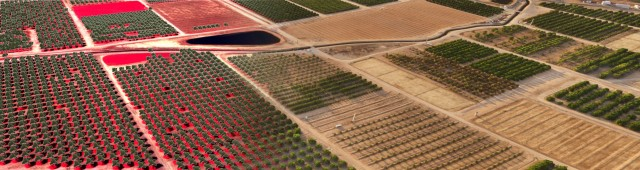
\includegraphics{images/fld-gde-banner_640x170.jpg}

\hypertarget{introduction}{%
\chapter{Introduction}\label{introduction}}

Drone technology has advanced dramatically in the last decade, thanks to significant advances in navigation, engines, batteries, storage, proximity sensors, and payloads,..

\hypertarget{mission-planning}{%
\chapter{Mission Planning}\label{mission-planning}}

\hypertarget{how-many-flights-will-it-take}{%
\section{How many flights will it take?}\label{how-many-flights-will-it-take}}

\hypertarget{tools-for-mission-planning}{%
\section{Tools for Mission Planning}\label{tools-for-mission-planning}}

\hypertarget{flight-operations}{%
\chapter{Flight Operations}\label{flight-operations}}

\hypertarget{crew-coordination}{%
\section{Crew Coordination}\label{crew-coordination}}

\hypertarget{check-lists}{%
\section{Check-Lists}\label{check-lists}}

\hypertarget{equipment}{%
\chapter{Equipment}\label{equipment}}

\hypertarget{accessories}{%
\section{Accessories}\label{accessories}}

\hypertarget{accessories-for-a-fixed-wing-mission}{%
\subsection{Accessories for a Fixed-wing Mission}\label{accessories-for-a-fixed-wing-mission}}

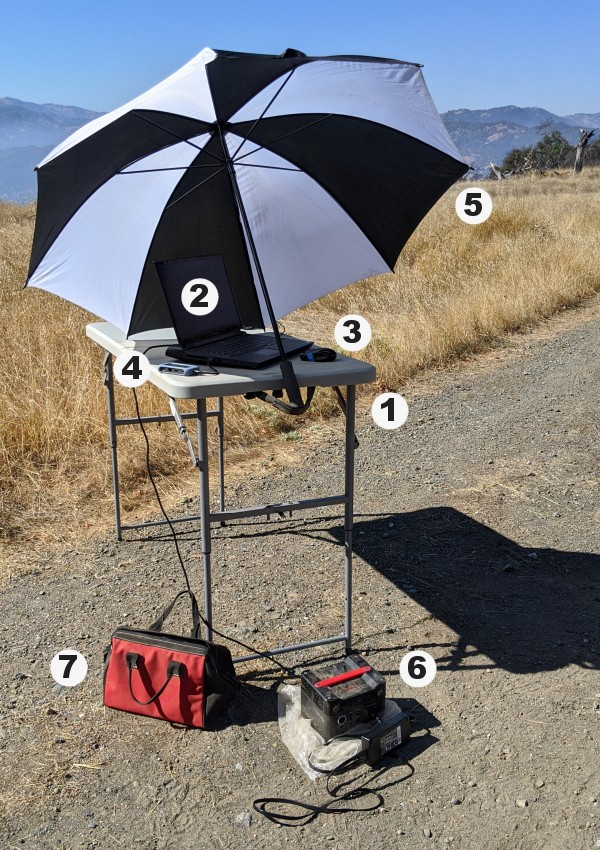
\includegraphics{images/accessories-ebee-labels_600x850.jpg}

\begin{enumerate}
\def\labelenumi{\arabic{enumi}.}
\tightlist
\item
  folding table
\item
  laptop for the flight management software (eMotion)
\item
  mouse
\item
  memory card reader
\item
  umbrella to keep the laptop cool and screen more visible
\item
  250W portable power station (big battery pack)
\item
  accessory bag with extra cables, memory cards, tools, etc.
\end{enumerate}

\hypertarget{accessories-for-a-quadcopter}{%
\subsection{Accessories for a Quadcopter}\label{accessories-for-a-quadcopter}}

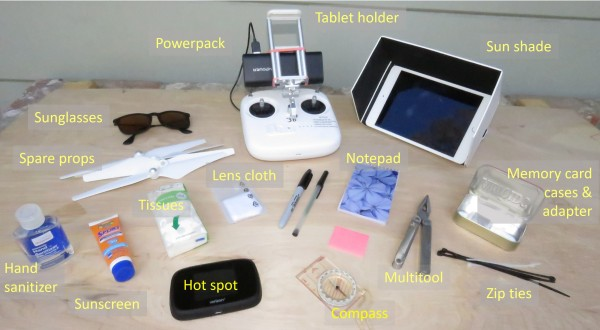
\includegraphics{images/accessories_with_labels_600x330.jpg}
\#\# Memory Cards

\hypertarget{how-many-memory-cards-do-i-need}{%
\subsection{How many memory cards do I need?}\label{how-many-memory-cards-do-i-need}}

Aim for enough memory cards for the number of flights you need to do each day. This way, you don't have to reformat the memory cards between flights, and the memory cards can serve as backup until you've got them backed-up on another storage device.

We like 32GB memory cards, because they're relatively cheap and have more than enough capacity to hold all the images from a single flight, even if its a multi-spectral camera mounted on a fixed wing drone. Look for memory cards that have a fast read-write rate, and avoid low end generic brands.

\hypertarget{keeping-memory-cards-organized}{%
\subsection{Keeping Memory Cards Organized}\label{keeping-memory-cards-organized}}

Typically when the drone lands you pull off the memory card and give it to someone who is in charge of the precious data. After a couple of flights, there are a bunch of memory cards sitting on someone's laptop, pocket, etc. and they all start to look the same. Sharpies, stickers, labels, and cases can help keep this organized and make sure they don't mixed up or accidentally erased.

\emph{photo here of memory card cases / labels / holders. }

\hypertarget{data-management}{%
\chapter{Data Management}\label{data-management}}

\hypertarget{diy-data-management-vs-one-stop-shops}{%
\section{DIY Data Management vs One-Stop Shops}\label{diy-data-management-vs-one-stop-shops}}

\hypertarget{moving-data-tools-of-the-trade}{%
\section{Moving Data: Tools of the Trade}\label{moving-data-tools-of-the-trade}}

\hypertarget{organizing-data-through-directory-trees}{%
\section{Organizing Data through Directory Trees}\label{organizing-data-through-directory-trees}}

\hypertarget{memory-cards---tips-and-tricks}{%
\section{Memory Cards - Tips and Tricks}\label{memory-cards---tips-and-tricks}}

\hypertarget{cataloging-data-making-it-findable}{%
\section{Cataloging Data \& Making it Findable}\label{cataloging-data-making-it-findable}}

\hypertarget{planning-a-drone-mapping-campaign}{%
\chapter{Planning a Drone Mapping Campaign}\label{planning-a-drone-mapping-campaign}}

by Andy Lyons, Shane Feirer, Becca Fenwick, and Sean Hogan

\hypertarget{introduction}{%
\section{Introduction}\label{introduction}}

Imagine yourself the Director of a nature reserve. You get an email - an instructor of a field methods class at the local university is offering to send you a group of graduate students to spend a week at your reserve to map the entire property with drones. That's an offer that's hard to pass up, but how do you even start to plan such a campaign? Mapping even a modest area with a single drone and a single pilot is a complicated workflow with a lot of moving parts. Coordinating multiple teams with multiple drones within a fix time frame adds even more complexity - particularly if you want to get good data!

This chapter offers some thoughts and suggestions for planning a drone campaign spanning multiple days and/or multiple flight teams. These lessons are based on our collective experiences including two campaigns to map \textgreater2000 acres of the Hopland Research and Extension Center, a xxx acre reserve in Mendicino County, California, most of which is extremely hilly oak woodland.

\hypertarget{staffing-rules-of-thumb}{%
\section{Staffing Rules of Thumb}\label{staffing-rules-of-thumb}}

When thinking about how many people you'll need (or conversely how many flight teams you can support), a general rule of thumb is to allocate a minimum of \textbf{two people per drone}.

At least one of person in each flight team needs to be an experienced drone pilot who holds a \textbf{FAA Part 107 Remote Pilot} license and is familiar with the equipment. In addition, each pilot will need at least one assistant to help with the many other tasks during fieldwork: packing and unpacking equipment, helping with launch and landing, keeping an eye open for any hazards in the air or on the ground, transferring and checking data, dealing with onlookers, etc.

In theory a single pilot could perform all the tasks themselves, but you want your pilot to not be frazzled so they can focus on what they do best: mission planning, controlling the flight, monitoring equipment status, and thinking about the overall safety environment.

If the assistant(s) are \textbf{novices}, having \textbf{two assistants per flight team} would be wise, at least for the first couple days of the campaign. If multiple teams are operating from a single launch site, you might be able to share an assistant across flights, but only if they're fairly experienced and physically fit!

It goes without saying that communication within a flight team is critical, and each team should do some practice flights \emph{before} you're actually collecting the research data. Two-way radios are frequently helpful particularly if someone needs to deploy GCPs or you need to walk to the launch location.

If you have the luxury of enough people, it can be helpful to appoint the most experienced person to be the \textbf{overall coordinator}. This person should under-occupied with flight responsibilities so they can keep an eye on what's coming up next, make sure important steps have not been forgotten, help troubleshoot technical issues, answer questions, keep an eye on the weather and the time, etc. The more moving parts you have in your field logistics, the more important it is to have someone in a coordinator role.

Another role you may want to consider delegating is \textbf{collecting media material}. These are your drone video shots, photos of the drones and flight crews, 360 panoramas, etc. Field assistants can perform these roles if they have the right experience, but be wary of asking your pilots to use the research drones to take media shots. Drone mapping and videography are often different skillsets and there's more than enough to deal with just managing mapping missions.

\hypertarget{planning-schedule}{%
\section{Planning Schedule}\label{planning-schedule}}

\hypertarget{months-before-the-campaign}{%
\subsection{2-3 months before the campaign}\label{months-before-the-campaign}}

Planning any kind of drone mapping project starts with a clear articulation of 1) the \textbf{science questions}, and 2) \textbf{data requirements} (e.g., what kind of imagery is needed - RGB, multispectral, or thermal? How about the spatial resolution, geographic area of interest, spatial accuracy, time of day). Check in with the research scientist(s) and/or land managers for clarification. If no one can articulate these basic requirements, consider that a \textbf{yellow flag} that you may be heading down the path of collecting data for the sake of collecting data! Rethink the project, or put it on hold until you're sure there's actually a need for the data.

2-3 months out is also when you want to assess \textbf{regulatory requirements}. If needed, start the process to apply for \textbf{FAA ATC clearance} or \textbf{Part 107 waviers}. Contact the \textbf{land manager} and start any permit processes required. Don't forget about contacting neighboring land owners, whose consent may not be strictly required but could prevent all manner of delays and disruptions to the project.

You also want to inventory your \textbf{equipment}. Don't forget \protect\hyperlink{accessories}{accessories} including enough batteries, memory cards, spare propellors, launch pads, field tables, pop-up shade structures, power supplies, cables, radios, first aid kit, fire extinguishers, water sprayers, etc. Give yourself enough time to order anything that's needed.

\hypertarget{weeks-before-the-campaign}{%
\subsection{2-4 weeks before the campaign}\label{weeks-before-the-campaign}}

Fine-tune the fieldwork logistics by doing a \textbf{reconnaissance of the area}. Identify launch sites, flight areas, travel times, etc. Finalize your estimate of the number of days / people / vehicles needed.

Prepare everything you need for the crew \textbf{training and orientation sessions}. These include printed maps of the project area with launch sites marked out, printed copies of any permits needed, phone numbers, equipment user guides, checklists, etc.

And don't forget your digital resources, which could include KMLs for the flight planning software, custom basemaps for Avenza Maps, soft copies of users guides, etc.

\hypertarget{week-before-the-campaign}{%
\subsection{1-week before the campaign}\label{week-before-the-campaign}}

\textbf{Training}. If possible, do your \textbf{test flights} and \textbf{training} with the field teams a week before the actual campaign. You want the trial and learning period to be \emph{before} the campaign so it is low-stress and the pressure of meeting a actual data collection schedule isn't pushing people to do things beyond their skill level.

Training the flight teams before the campaign starts will also give you a buffer to deal with equipment issues, evaluate if your campaign schedule is realistic, collect and process some sample data, tweak the parameters of your mission plans, and give your flight teams a chance to work together. You want your people to make mistakes during training, not the actual data collection.

\begin{quote}
You want your people to make mistakes during training,You want your people to make mistakes during training, not the actual data collection, not the actual data collection.
\end{quote}

Don't forget to practice \textbf{responding to the unexpected}. For example, if the drone lands off-target, or even worse drops out of the sky 1000 feet away, how are you going to organize a search and rescue operation? Practice loss of connection scenarios, test that your obstacle avoidance features actually work, etc. Even experienced pilots will benefit from this kind of refresher.

If it isn't possible to hold training and orientation prior to the campaign, plan on spending at least half of the first day on instruction, and at least half of the second day going over the data and debriefing the field work. You may not get as much research data collected those first two days, but by investing the time in instruction and reflection you'll be well on your way to a smooth and efficient operation.

\textbf{Weather}. Check the 10-day weather forecast

\hypertarget{week-of-the-campaign}{%
\section{Week of the Campaign}\label{week-of-the-campaign}}

\hypertarget{day-to-day-schedule}{%
\subsection{Day-to-day Schedule}\label{day-to-day-schedule}}

Many of us are used to waking up early during fieldwork, heading out to the site as quickly as possible, spending as much time as we can collecting data, returning to base when the sun goes down or our energy is depleted, having dinner, sleeping, waking up, and repeating.

However spending dawn-to-dusk in the field is a poor strategy for drone mapping. Shadows in the early morning and late afternoon can ruin data, so in most cases you really only want to fly a couple of hours before and after solar noon. However equally important, you need to allocate time to review and organize your data, and attend to the myriad tasks that come before and after flights.

After each day of flying, expect to spend \textbf{2-4 hours} copying and organizing the images into directories, downloading flight logs from your drones and GPS devices, typing up notes, post-processing data with your flight management software, creating metadata, doing some preliminary stitching for quality control, and refining the flight plans for the following day. Then there will also be a host of equipment tasks - dusting off lenses and engines, reformatting memory cards, recharging batteries, cleaning vehicles, etc. If the day didn't go great, you'll probably want to have a meeting with the flight team to process lessons learned and come up with a strategy to improve operations tomorrow.

If it isn't practical to work an additional 2-4 more hours at the end of each day in the field, then schedule an office day between flight days, or just plan on only spending 1/2 of each day flying. You may of course try to cram in as many flights per day, but at the risk of collecting data that doesn't stitch well, has gaps, or takes many extra hours of manual steps during processing.

\end{document}
